\documentclass[10pt]{article}
\usepackage{fullpage}
\usepackage{graphicx}
\usepackage{amssymb}
\usepackage{qtree}
\newcommand{\tab}{\hspace*{2em}}
\newcommand{\tabb}{\hspace*{4em}}
\newcommand{\tabbb}{\hspace*{6em}}
\begin{document}
	\begin{flushright}
	Lindsey Bieda and Joe Frambach\\
	Dynamic Programming Problems\\
	9.22.2011
	\end{flushright}
	\noindent
	7.  Give an efficient algorithm for the following problem. The input is an n sided convex polygon. Assume
			that the polygon is specified by the Cartesian coordinates of its vertices.  The output should be the
			triangulation of the polygon into n - 2 triangles that minimizes the sums of the perimeters of the
			into triangles. Note that this is equivalent to minimizing the length of the cuts required to create the
			triangle.\\
			\\
			Given an input of an array of points in clockwise order that form a convex polygon.\\
			\\
			\textbf{Recursive algorithm:}\\
				$minPerim(p_1,p_2,\ldots,p_n):$\\
				\\
				\tab base case: if n=3 return $\left\|p_1+p_2\right\|+\left\|p_2+p_3\right\|+\left\|p_1+p_3\right\|$\\
				\tab otherwise: return \[
				\min_{1 \leq x \leq n}(
						\underbrace{\left\|p_{x-1}+p_x\right\|+\left\|p_x+p_{x+1}\right\|+\left\|p_{x-1}+p_{x+1}\right\|}_{Perimeter~of~triangle~defined~by~x}
						~+~
						\underbrace{minPerim(I \setminus p_{x}}_{Remaining~polygon}~)
				)\]
				
				\begin{figure}[h]
					\centering
						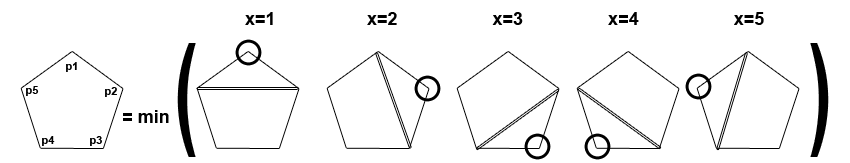
\includegraphics[width=450px]{dynamic7r.png}
					\caption{Illustration of the recursive call}
				\end{figure}\\
				\\
				The folowing is a conversion of the recursive solution into a bottom-up iterative solution for input $I$.\\
				\\
				1. Calculate Sbase Cases first:\\
				\tab For $T = [i_1, i_2, i_3]$ in $n \choose 3$, $i_1 < i_2 < i_3$: (that is, for every triangle permutation in $I$)\\
				\tabb Lookup[$T$] = $\left\|i_1+i_2\right\|+\left\|i_2+i_3\right\|+\left\|i_1+i_3\right\|$. (the perimeter of the triangle)\\
				\\
				2. Iterate!\\
				\tab For $m = 4$ to $n$: (Start with 4-gons, then 5-gons, \ldots, to $n$-gons)\\
				\tabb For $M = [i_1, i_2, i_3, \ldots, i_m]$ in $n \choose m$: (For every $m$-gon)\\
				\tabbb $Lookup(M) =$
				\[{\underbrace{\min_{1 \leq x \leq m}}_{See~Figure~1}~(~
					\underbrace{\left\|i_{x-1}+i_x\right\|+\left\|i_x+i_{x+1}\right\|+\left\|i_{x-1}+i_{x+1}\right\|}_{Perimeter~of~triangle~defined~by~x}
					~+~
					\underbrace{Lookup(M \setminus i_{x})}_{Remaining~m-1-gon}~)
					}_{modulo~m+1}\]\\
				\\
				3. Find solution.\\
				\tab The solution to the $n$-gon is at Lookup[$I$].
				
\end{document}